\documentclass[12pt,a4paper,bibliography=totocnumbered,listof=totocnumbered]{scrartcl}
%\documentclass[12pt,a4paper]{article}
\usepackage[ngerman]{babel}
\usepackage[utf8]{inputenc}
\usepackage{amsmath}
\usepackage{amsfonts}
\usepackage{amssymb}
\usepackage{graphicx}
\usepackage{fancyhdr}
\usepackage{tabularx}
\usepackage{geometry}
\usepackage{setspace}
\usepackage[right]{eurosym}
\usepackage[printonlyused]{acronym}
\usepackage{subfig}
\usepackage{floatflt}
\usepackage[usenames,dvipsnames]{color}
\usepackage{colortbl}
\usepackage{paralist}
\usepackage{array}
\usepackage{titlesec}
\usepackage{parskip}
\usepackage[right]{eurosym}
\usepackage[subfigure,titles]{tocloft}
\usepackage[pdfpagelabels=true]{hyperref}

\usepackage{listings}
\lstset{basicstyle=\footnotesize, captionpos=b, breaklines=true, showstringspaces=false, tabsize=2, frame=lines, numbers=left, numberstyle=\tiny, xleftmargin=2em, framexleftmargin=2em}
\makeatletter
\def\l@lstlisting#1#2{\@dottedtocline{1}{0em}{1em}{\hspace{1,5em} Lst. #1}{#2}}
\makeatother

\geometry{a4paper, top=27mm, left=20mm, right=20mm, bottom=35mm, headsep=10mm, footskip=12mm}


\hypersetup{unicode=false, pdftoolbar=true, pdfmenubar=true, pdffitwindow=false, pdfstartview={FitH},
	pdftitle={Wahlpflichtfach: Projekt: Client-K.I.s (ReversiXT, SS \the\year)},
	pdfauthor={Dr.\ Carsten Kern},
	pdfsubject={Projektbericht},
	pdfcreator={\LaTeX\ with package \flqq hyperref\frqq},
	pdfproducer={pdfTeX \the\pdftexversion.\pdftexrevision},
	pdfkeywords={Projektbericht, ReversiXT},
	pdfnewwindow=true,
	colorlinks=true,linkcolor=black,citecolor=black,filecolor=magenta,urlcolor=black}
\pdfinfo{/CreationDate (D:20151500000000)}
\titlespacing{\section}{0pt}{12pt plus 4pt minus 2pt}{-6pt plus 2pt minus 2pt}

% Kopf- und Fusszeile
\renewcommand{\sectionmark}[1]{\markright{#1}}
\renewcommand{\leftmark}{\rightmark}
\pagestyle{fancy}
\lhead{}
\chead{}
\rhead{\thesection\space\contentsname}
\lfoot{Implementierung von Brettspielen am Beispiel ReversiXT -- SS \the\year}
\cfoot{}
\rfoot{\ \linebreak Seite \thepage}
\renewcommand{\headrulewidth}{0.4pt}
\renewcommand{\footrulewidth}{0.4pt}

% Vorspann
\renewcommand{\thesection}{\Roman{section}}
\renewcommand{\theHsection}{\Roman{section}}
\pagenumbering{Roman}

\newcommand{\folgen}[1]{
\ensuremath
#1
}

\newcommand{\MyTitlepage}[5][\empty]{
\thispagestyle{empty}
\begin{center}
	
\includegraphics[scale=0.2]{pics/oth-logo.png}\\
	\vspace*{2cm}
	\Large
	\textbf{Fakultät}\\
	\textbf{Informatik und Mathematik}\\
	\vspace*{2cm}
	\Huge
	\textbf{Projektbericht}\\
	\vspace*{0.5cm}
	\large
	zum Wahlpflichtfach im SS \the\year\\
	\vspace*{1cm}
	\textbf{Projekt: Client-K.I.s (ReversiXT)}\\
	\vspace*{1cm}
	\includegraphics[height=6cm]{#1}
	\vfill
	\normalsize
	%\newcolumntype{x}[1]{>{\raggedleft\arraybackslash\hspace{0pt}}p{#1}}
	\begin{tabular}{rl}%{6cm}p{7.5cm}}
	    \rule{0mm}{5ex}\textbf{Gruppe:} & #2 \\
		\rule{0mm}{5ex}\textbf{Autoren:} & \hspace*{-0.5em}\begin{tabular}[t]{r}#3\end{tabular} \\ 
		\rule{0mm}{5ex}\textbf{Leiter:} & Prof. Dr. rer. nat. Carsten Kern \\ 
		\rule{0mm}{5ex}\textbf{Abgabedatum:} & #4 \\ 
	\end{tabular} 
\end{center}
\pagebreak
}

\begin{document}


% ----------------------------------------------------------------------------------------------------------
% Titelseite
% ----------------------------------------------------------------------------------------------------------
\MyTitlepage[pics/gamefield02]{07}{
\texttt{Katharina.Greim@st.oth-regensburg.de}\\
\texttt{Florian.Klamer@st.oth-regensburg.de}\\
\texttt{Tim.Lechner@st.oth-regensburg.de}}
{??.??.\the\year} % FIXME optional: Gruppenlogo als PNG, Pflichtfelder: Gruppe, Authoren durch "\\" getrennt und Abgabedatum eingeben

\setcounter{page}{1} 
% ----------------------------------------------------------------------------------------------------------
% Inhaltsverzeichnis
% ----------------------------------------------------------------------------------------------------------
\tableofcontents
\pagebreak


% ----------------------------------------------------------------------------------------------------------
% Inhalt
% ----------------------------------------------------------------------------------------------------------
% Abstände Überschrift
\titlespacing{\section}{0pt}{12pt plus 4pt minus 2pt}{-6pt plus 2pt minus 2pt}
\titlespacing{\subsection}{0pt}{12pt plus 4pt minus 2pt}{-6pt plus 2pt minus 2pt}
\titlespacing{\subsubsection}{0pt}{12pt plus 4pt minus 2pt}{-6pt plus 2pt minus 2pt}

% Kopfzeile
\renewcommand{\sectionmark}[1]{\markright{#1}}
\renewcommand{\subsectionmark}[1]{}
\renewcommand{\subsubsectionmark}[1]{}
\lhead{Kapitel \thesection}
\rhead{\rightmark}

\onehalfspacing
\renewcommand{\thesection}{\arabic{section}}
\renewcommand{\theHsection}{\arabic{section}}
\setcounter{section}{0}
\pagenumbering{arabic}
\setcounter{page}{1}

% ----------------------------------------------------------------------------------
% Kapitel: Einleitung
% ----------------------------------------------------------------------------------
\section{Einleitung}

%Leiten Sie in diesem Abschnitt in das Fach YIMB und das zu erstellende Projekt ein. %Beschreiben Sie kurz die Fragestellung, die in diesem Wahlpflichtfach gelöst werden %soll. Stellen Sie Ihr vorhandenes Vorwissen dar, das in dieser Veranstaltung für Sie %von Nutzen sein könnte/ist/war, etc.

Dieses Projekt basiert auf Reversi, ein ca. 100 Jahre altes Brettspiel. Ursprünglich ist es ein Spiel, bei dem zwei Spieler auf einem 8x8 großen Spielfeld um den Sieg fechten. Durch abwechselndes Legen von Spielsteinen versucht man so viel Fläche wie möglich zu besetzten. Der Kniff dabei ist, dass vom Gegner eingefärbte Felder durch geschicktes platzieren eigener Steine wieder invertiert werden können, daher auch der Name Reversi.

%TODO Reversi und ReversiXt bilder
Wie anfangs schon erwähnt, hat die Standartversion von Reversi ein relativ kleines Spielfeld und nur zwei Spieler. Es gibt nur zwei Arten von Spielsteinen, nämlich die der zwei Spieler. Das steht im starken Kontrast zu ReversiXT, für das dieses Projekt eine KI entwickelt. In der erweiterten Version des Spiels, sind bis zu acht Spieler erlaubt. Außerdem gibt einige Sonder-Spielsteine und Felder. Diese Steine bestehen aus \glqq Überschreibsteinen\grqq, die es ermöglichen gegnerische Spielsteine umzufärben und \glqq Bomben\grqq. Mit diesen kann man in der zweiten Phase des Spiels Bereiche des Spielbretts zerstören. Dazu folgt später mehr. Die neuen Spielfelder sind \glqq Wahlfeld\grqq{} (choice)(c), welches es dem besetzenden Spieler ermöglicht, mit einem Mitspieler seiner Wahl Spielsteine zu tauschen (auch mit sich selbst). \glqq Inversionsfelder\grqq (inversion)(i), wenn aktiviert, verschieben die Spielerfarben um eins. Besetzt ein Spieler ein \glqq Bonusfeld\grqq (bonus)(b) so hat er die Möglichkeit eine extra Bombe oder einen extra Überschreibstein zu erhalten. Zuletzt gibt es noch \glqq Expansionsfelder\grqq (expansion)(x). Diese agieren wie \glqq tote\grqq{} Spieler und können durch normale Züge oder das Platzieren von Überschreibsteinen eingefärbt werden.

Unsere Aufgabe in diesem Projekt ist es, einen künstlichen-Intelligenz Spieler Clienten zu programmieren. Dieser soll gegen andere KIs auf einem, von einem Server gehostetem Spiel antreten. Grundvoraussetzung ist natürlich, dass die KI nur gültige Züge berechnet und einer von uns entwickelten Heuristik folgt. Diese Heuristik ist das Herzstück des Projekts. Sie ist maßgeblich dafür verantwortlich, gute Zugentscheidungen zu treffen und schließlich das Spiel zu gewinnen. All die oben genannten Schritten sind Vorbereitung für einen großen Wettkampf gegen Ende des Semesters. In der Endphase des Wahlpflichtmoduls findet nämlich ein virtueller Wettstreit zwischen den KIs der Studenten der RWTH Aachen und der OTH Regensburg statt. Historisch ist die OTH schon oft als Sieger hervorgegangen und wir hoffen auch dieses Jahr auf einen Sieg.

Insgesamt sieht unser Team dieses Projekt als gute Lernmöglichkeit um unsere Programmier-, Team- und weitere Fähigkeiten zu erweitern. Wir kommen alle mit relativ wenig Erfahrung in dieses Projekt und hoffen deswegen, die oben genannten und viele weitere Dinge zu vertiefen.

\newpage
% ----------------------------------------------------------------------------------
% Kapitel: Allgemeine Informationen
% ----------------------------------------------------------------------------------
\section{Allgemeine Informationen}

In diesem Teil werden die technischen und sozialen Rahmenbedingungen des Projekts erläutert und weitere allgemeine Informationen dargelegt. Das soll helfen, das Projekt und alle Beteiligten daran in Perspektive zu setzten. Außerdem können so Entscheidungen über verwendete Technologien aus Sicht des Teams besser nachvollziehbar gemacht werden. Die Vorstellung des Teams eröffnet dieses Kapitel und wird gefolgt von der Beschreibungen der eingesetzten Software sowie der verwendeten Datenstruktur die zur Speicherung des Spielfeldes und verbundenen Daten dient.

\subsection{Team und Kommunikation}
%Beschreiben Sie in diesem Abschnitt Ihr Team. Welche Person hat welche Aufgaben %wahrgenommen, wie wurden Aufgaben aufgeteilt und wie wurde kommuniziert, etc.
Alle aus dem Team befinden sich gerade im 4. Semester der allgemeinen Informatik. Daher kennen wir uns bereits aus den letzten Semestern uns sehen uns häufig in den Vorlesungen, wodurch ein Großteil der Kommunikation im Team bereits dort stattfindet. Zusätzlich stehen wir über Whats-App, die Gruppenmailingliste und über das lokale Gruppen-Repository in Kontakt.

Obwohl das Team im gleichen Studiengang ist hat jedes Teammitglied natürlich einen eigenen Werdegang und damit auch andere Erfahrungen und Fähigkeiten. Diese werden in diesem Abschnitt nun im Zusammenhang zum Projekt erläutert.

%TODO Alle genauer erklären für was bestimmte Vrkenntnisse im Projekt konkret wichtig sind
Katharina Greim hat in den ersten drei Semestern ihres Studiums Programmierkenntnisse in Java und C erlernt. In den Vorlesungen Mathematik 1 \& 2 und Algorithmen \& Datenstrukturen wurde das Lösen von abstrakten Problemen und Implementieren von verschiedenen Datenstrukturen oft geübt. Da Sie zusätzlich ein Tutorium hält, hat sie gelernt, individuell auf Menschen einzugehen und komplizierte Dinge leicht verständlich zu erklären, was bei der Arbeit im Team sehr hilfreich sein wird. Außerdem hat sie bereits einige Erfahrungen mit \LaTeX\quad gesammelt. 

Florian Klamer hat Vorkenntnisse aus früheren Vorlesungen wie Programmieren 1 \& 2 die grundsätzlich wichtig für die Implementierung und Strukturierung der KI sind. Aus Algorithmen und Datenstrukturen sind die Teile wichtig, bei denen es um effiziente und sichere Algorithmen für z.B die Berechnung der Heuristik oder der gültigen Züge geht. Neben dem Studium hilft Florian außerdem ehrenamtlich beim Connecta e.V. mit. Dort ist er im EDV Ressort mit der Betreuung des Intra-, Extranets, der Datenbank und der Webseite beschäftigt. Die dort erworbenen Fähigkeiten sind z.B. in Git, SQL oder Teamarbeit, können aber ebenso wichtig für das Projekt sein.

Tim Lechner hat die für das Projekt erforderlichen Vorkenntnisse aus früheren Vorlesungen wie Programmieren 1 \& 2, Algorithmen und Datenstrukturen erworben.

 Der letzte Teil in diesem Abschnitt ist eine Liste (Tabelle 1) der Übungsaufgaben und von wem sie bearbeitet wurden.

%TODO Tabelle vervollständigen
\begin{table}[]
	\centering
	\caption{Aufgabenverteilung}
	\label{my-label}
	\begin{tabular}{|l|l|l|}
		\hline
		Übung & Bearbeiter & Kommentar \\ \hline
		1               & Flo        & Test      \\ \hline
		2               &            &           \\ \hline
		3               &            &           \\ \hline
		4&            &           \\ \hline
		5&            &           \\ \hline
		6&            &           \\ \hline
				7&            &           \\ \hline
		8&            &           \\ \hline
		9&            &           \\ \hline
	\end{tabular}
\end{table}

\subsection{Technische Daten}
%Beschreiben Sie u.a.\ in welcher Programmiersprache und unter welchem Betriebssystem Sie entwickeln, welche IDEs Sie nutzen, welche zusätzlichen Tools bei Ihrer Projektentwicklung Einsatz gefunden haben, etc.

Die Implementierung gestaltet unser Team mit Java 9. Das ist eine der Sprachen, die unser Team im Studium gelernt hat und am besten beherrscht. Als Betriebssystem verwenden wir alle hauptsächlich Windows 10. Manchmal, vor allem zum Testen, kommt auch Linux (Ubuntu)(Version 18.04?????) zum Einsatz. Im Team benutzen wir alle IntelliJ (Version 2018.1.3) von JetBrains. Diese IDE hat viele nützliche Features und ist für uns als Studenten für nicht kommerzielle Projekte kostenlos. Zum Testen unserer KI und zum einfacheren Bau eigener Karten benutzen wir das von Herr Kern zur Verfügung gestellte Kartenbauprogramm.
 Das letzte Tool zur Programmierung welches eingesetzt wird ist das Buildtool Gradle (Version 4.4 ?????). Es ist einfach zu benutzen und das Buildscript kann unter anderem durch den Einsatz einer eigenen Sprache namens Groovy kurz und kompakt gestaltet werden.
%TODO eventuelle weitere Software eintagen

Um unser Programm gegen andere KIs testen zu können, verwenden wir den zu Verfügung gestellten ReversiXT Server, der auch lokal funktioniert.
%TODO Server
%TODO Maptool

Dieser Projektbericht ist mit der Textsatzsystem LaTeX geschrieben. Hauptsächlich verwenden wir TeXstudio 2.12.8 als Editor, testen aber auch andere wie TeXworks, um die beste Arbeitsumgebung zu finden.

Die Rechner auf denen wir programmieren und testen sind vor allem \glqq Mittelklasselaptops\grqq. Um den Rahmen nicht zu sprengen, sind hier die genauen Namen zu den Geräten aufgelistet, wenn man noch weitere Details braucht. Florian benutzt ein Lenovo Yoga 720(2017) %TODO nummer raussuchen.
Katharina verwendet ein ....%TODO Name und nummer eintragen
Tim setzt ein ... ein.%TODO Name/nummer eintragen

\subsection{Datenstruktur}
%Beschreiben Sie die Datenstruktur, die Sie zur Speicherung des Spielfeldes in Ihrem %Client nutzen. Gehen Sie auf Besonderheiten ein und erklären Sie, wie diese %funktionieren und was Sie sich davon erhoffen. Geben Sie falls möglich auch eine %schematische Darstellung/ein Bild der Datenstruktur an.
Im ersten Versuch der Datenstruktur wurde die Anzahl der Spieler, Bomben, die Stärke usw. in Integer Variablen und das Spielfeld in einem String Array abgespeichert. Da diese Version viel Speicherplatz und Rechenzeit benötigt, wird sie ab sofort noch verbessert.
Um die Datenstruktur zu verbessern, wollen wir folgende Punkte umsetzten:
\newline
1. Die Anzahl der Spieler, Überschreibsteine, Bomben sowie die Stärke der Bomben und die Spielfeldhöhe/-breite werden alle in Short Variablen gespeichert. 

Da die Anzahl der Spieler auf 8 begrenzt ist und auch das Spielfeld eine maximale Größe von 50 x 50 haben kann, reicht die Short Variable vollkommen aus. Auch für die Anzahl und Stärke der Bomben und Anzahl der Überschreibsteine wird die Größe eines Shorts genügen.

2. Das Spielfeld wird in einem zweidimensionalem Charakter Array gespeichert.

Da im Spielfeld nur einzelne Zeichen stehen, ist es sinnvoll einen Charakter und keinen String zu verwenden. Außerdem bietet sich ein Array sehr gut an, da die Höhe und Breite bereits vor dem Einlesen des Spielfeldes bekannt ist und somit sehr gut auf die einzelnen Felder zugegriffen werden kann.
Eine zusätzliche Erweiterung wäre ein dreidimensionales Array, bei dem zu jedem Spielfeld noch zusätzliche Informationen abgespeichert werden können, z.B. ob eine Transition an dieser Stelle vorhaben ist.

3. Die Transitionen werden so in einer Datenstruktur abgespeichert, dass eine schnelle Suche nach einer bestimmten Transition möglich ist. 

%TODO geeignete Datenstruktur für Transitionen nachtragen  

\newpage
% ----------------------------------------------------------------------------------
% Kapitel: Spielfeldbewertung
% ----------------------------------------------------------------------------------
\section{Spielfeldbewertung}
\subsection{Spielfeldbewertung: 1. Vorschlag}
%Beschreiben Sie wie in der zugehörigen Projektaufgabe gefordert eine erste Heuristik.
Die Heuristik soll einen vorliegenden, beliebigen Spielstand für einen gegebenen Spieler bewerten. Das bedeutet, es soll ermittelt werden, ob dieser Zustand für den Spieler besonders gut oder schlecht ist. Somit können Züge später danach ausgesucht werden, ob eine Reihe von Zügen zu einer besonders guten Situation für einen Spieler oder auch zu einer besonders schlechten Situation für einen Gegenspieler führen kann.  

Die grundlegende Idee der ersten Spielfeldbewertung ist, Spielfelder anhand ihrer 'Färbbarkeit' einzuschätzen. Als Hauptfaktor dient dazu wie schwer ein Feld vom Gegner umzufärben ist. Ist ein Feld z.B. nur noch von einer Seite einfärbbar, ist es sicherer als ein frei einfärbbares. Das bedeutet es bekommt eine bessere Bewertung. Wichtig ist außerdem die Beweglichkeit. Der Client soll das Spiel so lenken, dass er auf sicheren Steinen aufbauen kann, dabei aber nicht seine Mobilität, also die Anzahl an möglichen Zügen, verliert. In Summe führt das dazu, dass sich alle Spielsteine möglichst gegenseitig schützen.


Um die Färbarkeit zu beurteilen, wird die Färbung in folgende vier Richtungen geprüft:

1. horizontal - von links nach rechts oder umgekehrt \newline
2. vertikal - von oben nach unten oder umgekehrt \newline
3. von links oben nach rechts unten oder umgekehrt \newline
4. von rechts oben nach links unten oder umgekehrt \newline
	
Beispiel 1: Liegt ein Stein in einer Ecke, so ist es weder horizontal, vertikal oder schräg möglich diesen Stein umzufärben. Somit ist dieses Feld zu 0/4 einfärbbar und damit sehr wichtig.\newline 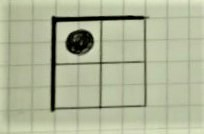
\includegraphics[height=2cm]{pics/beispiel1}

Beispiel 2: Liegt ein Stein am rechten Rand, so ist es möglich den Stein vertikal umzufärben, aber nicht horizontal oder schräg. Somit ist dieses Feld zu 1/4 einfärbbar und somit wichtig.\newline

\includegraphics[height=2cm]{pics/beispiel2}

Beispiel 3: Liegt ein Stein innerhalb des Spielfeldes, so ist es möglich den Stein horizontal, vertikal und schräg einzufärben. Somit ist dieses Feld zu 4/4 einfärbbar und damit nicht so wichtig.\newline
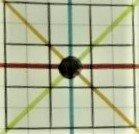
\includegraphics[height=2cm]{pics/beispiel3}
\newpage
Beispiel 4: Liegt ein Stein innerhalb des Spielfeldes und zusätzlich ist links oben (Transitionenrichtung 7) ein Stein der selben Farbe der zu 0/4 einfärbbar ist, dann ist der Stein von links oben nach rechts unten und umgekehrt nicht einfärbbar. Somit ist dieses Feld zu 3/4 einfärbbar und damit wichtiger als ein Feld wie in Beispiel 3.\newline
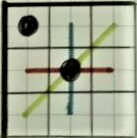
\includegraphics[height=2cm]{pics/beispiel4}

Mit dieser Bewertung kann sowohl die Situation um ein Einzelfeld herum, als auch Transitionen betrachtet werden. 

\subsection{Spielfeldbewertung: 2. Vorschlag}
Die Idee der zweiten Spielfeldbewertung ist die eigene Mobilität einzuschätzen. Denn wenn man nur sehr wenige Möglichkeiten hat einen Zug zu machen kann der Gegner bestimmen wo man hinsetzten muss und hat selbst keinen oder nur einen geringen einfluss auf den Spielverlauf. Im schlimmsten Fall hat man gar keine Möglichkeit zu ziehen und ermöglicht so den Gegnern mehrmals zu färben wärend man nichts färben kann.

Hierbei ist zu beachten, dass der Sprung von einen möglichen Zug zu zwei möglichen Zügen eine größerer verbesserung ist als von 10 auf 20 mögliche Züge.
Zu Beginn eines Spieles hat man natürlich wenig Möglichkeiten Steine zu platzieren aber der Gegener hat auch nicht so viele Möglichkeiten Stein zu platzieren, so dass es schwierig ist den anderen Spieler zu gewissen Aktionen zu bewegen da alle Spieler eingeschränkt sind.Eine besonders schlechte Situation ist es also wenn ein feindlicher Spieler viele Zugmöglichkeiten hat wärend man selbst nur sehr wenige hat.

Beispiel 1: Hier hat Blau keinen Zug mehr Blau muss also aussetzen.
\newline
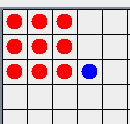
\includegraphics[height=2cm]{pics/BlauKeinZug}

Beispiel 2: Blau hat nur einen möglichen Zug er hat also keinen Einfluss auf das Spiel mehr, da er nichts entscheiden kann.
\newline
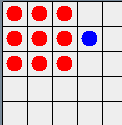
\includegraphics[height=2cm]{pics/BlauEinZug}

Beispiel 3: Blau hat sehr viele Möglichkeiten Steine zu platzieren. Obwohl Rot hier mehr steine hat befindet sich blau in einer sehr guten Position da Blau deutlich mehr Zugmöglichkeiten hat als Rot.
\newline
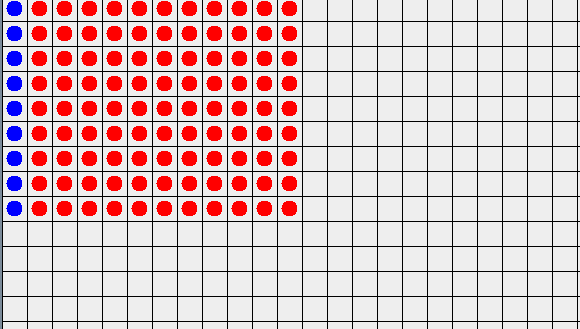
\includegraphics[height=2cm]{pics/BlauVieleZuege}
 
Die Art der Bewertung soll verhindern, dass man die Möglichkeit verpasst gegnerische Steine zu färben.








\subsection{Final implementierte Spielfeldbewertung}
Beschreiben Sie abschließend, welche Heuristik final in Ihrem Client umgesetzt ist. Beschreiben Sie dazu auch Werte von Parametern (Kriterien und Gewichtungen), die Sie in den einzelnen Implementierungen nutzen. Welche statischen Vorberechnungen Sie machen, um z.B.\ das Spielfeld zu analysieren, etc.


\newpage
% ----------------------------------------------------------------------------------
% Kapitel: Statistiken
% ----------------------------------------------------------------------------------
\section{Statistiken}
Integrieren Sie in diesen Abschnitt alle Ergebnisse von Projektaufgaben, die mit Erstellungen von Statistiken zu tun haben. Geben Sie dabei auch Diagramme an und interpretieren Sie die darin dargestellten Kurven. Beschreiben Sie zu jedem implementierten Verfahren, ob und welchen Nutzen es aus Ihrer Sicht gebracht hat.

\subsection{Vergleich ... und ...}

\subsection{Vergleich ..., ... und ...}

\subsection{...}


\newpage
% ----------------------------------------------------------------------------------
% Kapitel: Bombenphase
% ----------------------------------------------------------------------------------
\section{Bombenphase}
Beschreiben Sie, wie Sie Bomben werfen (z.\,B.\ die eingesetzte Bewertungsheuristik und, ob Sie in die Tiefe rechnen und falls ja, wie tief Sie rechnen)


\newpage
% ----------------------------------------------------------------------------------
% Kapitel: Eigene Spielfelder
% ----------------------------------------------------------------------------------
\section{Wettbewerbs-Spielfelder}
Beschreiben Sie in diesem Abschnitt die Spielfelder, die Sie für den Wettbewerb eingereicht haben/einreichen wollen. Fügen Sie in diesen Abschnitt auch die entsprechenden Bilder der Karten ein, geben Sie Zusatzinformationen wie Spieleranzahl, Bombenanzahl und -stärke, Anzahl Überschreibsteine etc.\ an.

Beschreiben Sie außerdem, warum sie die jeweiligen Karten eingereicht haben: in welcher Hinsicht versprechen Sie sich von den eingereichten Karten Vorteile; in wie weit sind diese Karten auf Ihren Client und die darin implementierte Heuristik zugeschnitten, etc.


\newpage
% ----------------------------------------------------------------------------------
% Kapitel: Fazit
% ----------------------------------------------------------------------------------
\section{Fazit}
Beschreiben Sie in diesem Abschnitt u.a.\ was Ihnen an diesem Fach gefallen hat und welche Verbesserungsvorschläge Sie für künftige Veranstaltungen haben. Was konnten Sie dazulernen, in welchen Bereichen haben Sie sich verbessert. Welche Problemsituationen gab es während der Projekterstellung, wie sind Sie diese angegangen und wie haben Sie diese gelöst. Was haben Sie evtl.\ vermisst.


\newpage
% ----------------------------------------------------------------------------------
% Kleine Einführung in LaTeX-Elemente
% ----------------------------------------------------------------------------------
\section{\LaTeX-Elemente}
Dieser Abschnitt soll nicht Bestandteil des Projektberichtes sein, sondern beinhaltet lediglich einige Informationen über \LaTeX-Distributionen, Editoren und \LaTeX-Elemente, die Ihnen beim Einstieg in das \LaTeX-Textsatzsystem helfen sollen.

\subsection{\LaTeX-Distributionen nach Betriebssystemen}

\subsubsection{\LaTeX-Distributionen}
Folgende Haupt-\LaTeX-Distributionen stehen Ihnen zur Verfügung:
\begin{itemize}
  \item Windows:\quad \texttt{MiKTeX}\quad Webseite:\quad\url{http://www.miktex.org}
  \item Linux/Unix:\quad \texttt{TeX Live}\quad Webseite:\quad\url{http://tug.org/texlive/}
  \item Mac OS:\quad \texttt{MacTeX}\quad Webseite:\quad\url{http://www.tug.org/mactex/}
\end{itemize}

\subsubsection{\LaTeX-Editoren}
Auf folgenden Webseiten können Sie einige hilfreiche \LaTeX-Editoren finden:
\begin{itemize}
  \item Windows/Linux/Mac OS: \url{http://www.xm1math.net/texmaker/}
  \item Windiws: \url{http://www.texniccenter.org/}
  \item Mac OS: \url{http://pages.uoregon.edu/koch/texshop/}
\end{itemize}

Falls bei den oben genannten Editoren kein passender vorhanden war, findet sich auf Wikipedia eine Zusammenstellung vieler weiterer \LaTeX-Editoren:\\[1em]
\hspace*{3cm}\url{https://en.wikipedia.org/wiki/Comparison_of_TeX_editors}


\subsection{Unterabschnitt}
Zum Einfügen eines Bildes, siehe Abbildung \ref{fig:reversi01}, wird die \textit{minipage}-Umgebung genutzt, da die Bilder so gut positioniert werden können.

\vspace{1em}
\begin{minipage}{\linewidth}
	\centering
	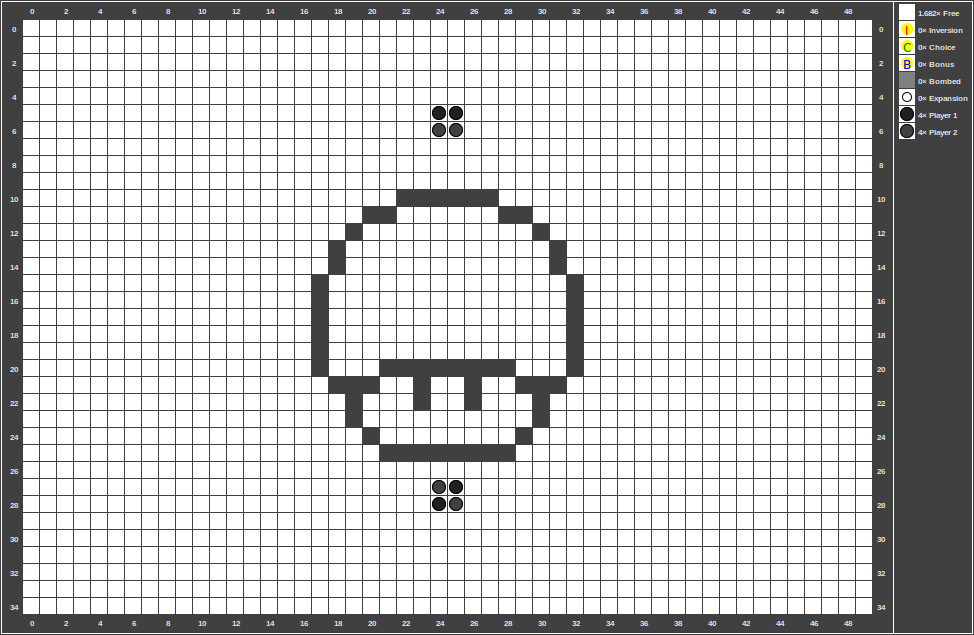
\includegraphics[width=0.6\linewidth]{pics/gamefield01.png}
	\captionof{figure}[Spielfeld 01]{Unbespieltes Spielfeld\footnotemark }
	\label{fig:reversi01}
\end{minipage}
\footnotetext{Diesem Spielfeld wurden noch keine Spieler zugewiesen (daher die dunklen Spielsteine)}

Nachdem das Spielt gestartet wurde und beiden Spielphasen durchlaufen wurden, siegt schließlich der Spieler mit der Farbe rot.

\vspace{1em}
\begin{minipage}{\linewidth}
	\centering
	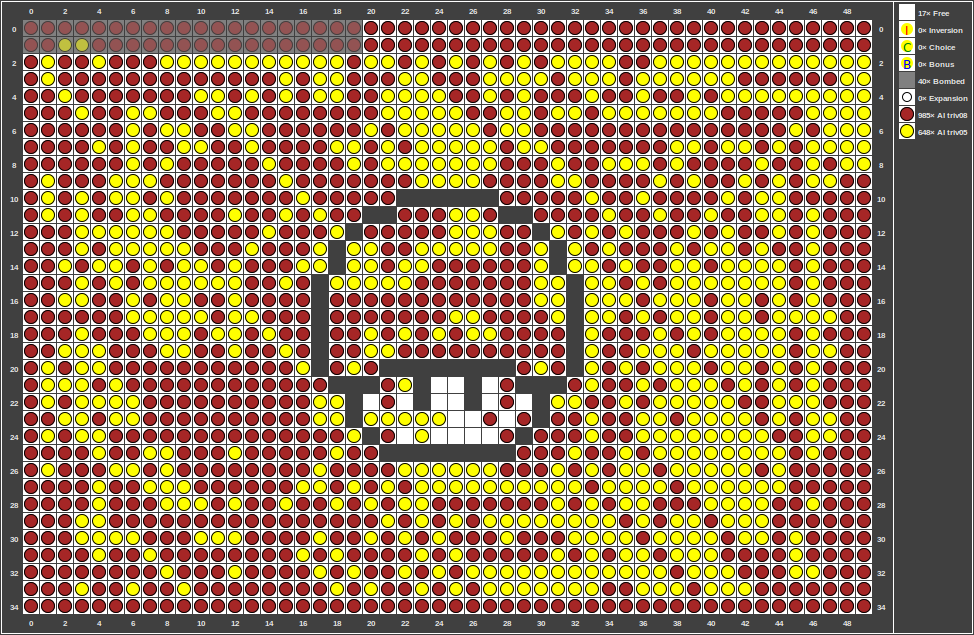
\includegraphics[width=0.6\linewidth]{pics/gamefield02.png}
	\captionof{figure}[Spielfeld 02]{Finales Spielfeld\footnotemark }
	\label{fig:reversi2}
\end{minipage}
\footnotetext{Das Spielfeld nach der Zug- und Bombenphase. Spieler rot gewinnt eindeutig.}

\subsection{Tabellen}
In diesem Abschnitt wird eine Tabelle (siehe Tabelle \ref{tab:beispiel}) dargestellt.

\vspace{1em}
\begin{table}[!h]
	\centering
	\begin{tabular}{|l|l|l|}
		\hline
		\textbf{Name} & \textbf{Name} & \textbf{Name}\\
		\hline
		1 & 2 & 3\\
		\hline
		4 & 5 & 6\\
		\hline
		7 & 8 & 9\\
		\hline
	\end{tabular}
	\caption{Beispieltabelle}
	\label{tab:beispiel}
\end{table}


\subsection{Auflistung}
Für Auflistungen wird die \textit{enumerate}- oder \textit{itemize}-Umgebung genutzt.

\begin{itemize}
	\item Nur
	\item ein
	\item Beispiel.
\end{itemize}

\subsection{Listings}
Zuletzt ein Beispiel für ein Listing, in dem Quellcode eingebunden werden kann, siehe Listing \ref{lst:arduino}.

\vspace{1em}
\begin{lstlisting}[caption=Arduino Beispielprogramm, label=lst:arduino]
int ledPin = 13;
void setup() {
    pinMode(ledPin, OUTPUT);
}
void loop() {
    digitalWrite(ledPin, HIGH);
    delay(500);
    digitalWrite(ledPin, LOW);
    delay(500);
}
\end{lstlisting}

\subsection{Tipps}
Die Quellen befinden sich in der Datei \textit{quellen.bib}. Eine Buch- und eine Online-Quelle sind beispielhaft eingefügt. [Vgl. \cite{buch}, \cite{online}]

\pagebreak

% ----------------------------------------------------------------------------------------------------------
% Kapitel
% ----------------------------------------------------------------------------------------------------------
\section{Kapitel}
Lorem ipsum dolor sit amet.

\subsection{Unterkapitel}
Lorem ipsum dolor sit amet, consetetur sadipscing elitr, sed diam nonumy eirmod tempor invidunt ut labore et dolore magna aliquyam erat, sed diam voluptua. At vero eos et accusam et justo duo dolores et ea rebum. Stet clita kasd gubergren, no sea takimata sanctus est Lorem ipsum dolor sit amet. Lorem ipsum dolor sit amet, consetetur sadipscing elitr, sed diam nonumy eirmod tempor invidunt ut labore et dolore magna aliquyam erat, sed diam voluptua. At vero eos et accusam et justo duo dolores et ea rebum. Stet clita kasd gubergren, no sea takimata sanctus est Lorem ipsum dolor sit amet.

\subsection{Unterkapitel}
Lorem ipsum dolor sit amet, consetetur sadipscing elitr, sed diam nonumy eirmod tempor invidunt ut labore et dolore magna aliquyam erat, sed diam voluptua. At vero eos et accusam et justo duo dolores et ea rebum. Stet clita kasd gubergren, no sea takimata sanctus est Lorem ipsum dolor sit amet. Lorem ipsum dolor sit amet, consetetur sadipscing elitr, sed diam nonumy eirmod tempor invidunt ut labore et dolore magna aliquyam erat, sed diam voluptua. At vero eos et accusam et justo duo dolores et ea rebum. Stet clita kasd gubergren, no sea takimata sanctus est Lorem ipsum dolor sit amet.
\pagebreak

% ----------------------------------------------------------------------------------------------------------
% Literatur
% ----------------------------------------------------------------------------------------------------------
\renewcommand\refname{Quellenverzeichnis}
\bibliographystyle{alpha}
\bibliography{quellen}
\pagebreak

% ----------------------------------------------------------------------------------------------------------
% Anhang
% ----------------------------------------------------------------------------------------------------------
\pagenumbering{Roman}
\setcounter{page}{1}
\lhead{Anhang \thesection}

\begin{appendix}
\section*{Anhang}
\phantomsection
\addcontentsline{toc}{section}{Anhang}
\addtocontents{toc}{\vspace{-0.5em}}

\section{GUI}
Ein toller Anhang.

\subsection*{Screenshot}
\label{app:screenshot}
Unterkategorie, die nicht im Inhaltsverzeichnis auftaucht.

\end{appendix}


\end{document}
